\documentclass[11pt]{article}
\input{\string~/.macros}
\usepackage[a4paper, total={6in, 8in}, margin=0.5in]{geometry}

\usepackage{graphicx}   % incorporating graphics
\graphicspath{{assets/}}

% arg1=pdfurl arg2=pagenum arg3=text
\usepackage{url}
\usepackage{hyperref}
\hypersetup{colorlinks=true, linktoc=all, linkcolor=blue}
\newcommand{\linkbook}[3][../fundamentals_of_computer_graphics_4ed.pdf]{
    \noindent\href[page=#2]{#1}{\urlstyle{rm}{#3}}
}

\newcommand{\heading}[1]{(#1)}
\newcommand{\bheading}[1]{\textbf{(#1)}}

\begin{document}
\linkbook{3}{table of contents}
\tableofcontents
\newpage


\section{\linkbook{12}{Introduction}}
\section{\linkbook{24}{Misc Math}}

\begin{enumerate}
    \item \bheading{\linkbook{30}{trig identities}}
    \item \bheading{dot product}
    \[
        \ba \cdot \bb = \norm{\ba} \norm{\bb} \cos \phi    
        \qquad
        proj_{\ba}(\bb)= \norm{\ba}\cos(\phi) = \frac{a\cdot b}{\norm{\bb}}
    \]
    \item \bheading{cross product}
    \[
        \ba \times \bb = \norm{\ba} \norm{\bb} \sin (\phi) \bn 
        = \det \begin{pmatrix}
            \bi & \bj & \bk \\
            a_1 & a_2 & a_3 \\
            b_1 & b_2 & b_3 \\
        \end{pmatrix}
    \]
    where $\bn$ is unit vector perpendicular to plane formed by $\ba,\bb$, determined by the right hand rule
    \item \bheading{coordinate frames}
    \begin{itemize}
        \item the \textbf{global coordinate system} is one formed by cartesian canonical orthonormal basis and the canonical origin that is not stored explicitly. 
        \item Other coordinate system is called a \textbf{frame of reference} or \textbf{coordinate frame} are stored explicitly (the origin, and 3 orthonormal vectors as a function of the canonical basis) and is called a \textbf{local coordinate system}
        \item If $\bb$ is in canonical $\bx-\by-\bz$ coordinate and want to transform to a local $\bu-\bv-\bw$ coordinate. then the transformed vecter can be written as 
        \[
            \sum_{\bq \in \pc{\bu,\bv,\bw}} \inner{\bq}{\bb} \bq
        \]
    \end{itemize}
    \item \bheading{construct basis} by Gram–Schmidt process
    \item \bheading{\linkbook{55}{linear interpolation}} over 2 points or a set of points where the function is piece-wise linear
    \item \bheading{\linkbook{55}{triangles}}
    \begin{itemize}
        \item barycentric coordinates is a nonorthogonal makes interpolation straight-forward over a triangle. Say $(\ba,\bb,\bc)$ forms a triangle, then the vertices $(\ba,\bb,\bc)$ act as basis vectors and form the barycentric coordinates. Any point $\bp$ is 
        \[
            \bp(\alpha,\beta,\gamma) = \alpha \ba + \beta \bb + \gamma \bc
            \quad \quad 
            \alpha+\beta+\gamma=1
        \]
        $(\alpha,\beta,\gamma)$ is the barycentric coordinate of $\bp$ w.r.t. $\ba,\bb,\bc$. Given $\bp$ in cartesian coordinate, we can find its baarycentric coordinate by solving
        \[
            \bp = \ba + \beta(\bb-\ba) + \gamma(\bc-\ba)
            \quad \iff \quad
            \begin{pmatrix}
                x_b - x_a & x_c - x_a \\
                y_b - y_a & y_c - y_a \\
            \end{pmatrix}    
            \begin{pmatrix}
                \beta \\ \gamma \\
            \end{pmatrix}
            = 
            \begin{pmatrix}
                x_p - x_a \\
                y_p - y_a \\
            \end{pmatrix}
        \]
        Geometrically, $\alpha,\beta,\gamma$ can be computed using triangle area
        \[
            \alpha = A_{\alpha}/A 
            \quad
            \beta = A_{\beta} / A
            \quad
            \gamma = A_{\gamma} /A    
        \]
        Properties
        \begin{itemize}
            \item can detect pointson edge/verties easily
            \item mixes coordinates of vertices smoothly
            \item can detect insidedness of points easily, i.e. $\alpha,\beta,\gamma > 0$
        \end{itemize}
    \end{itemize}
\end{enumerate}



\section{\linkbook{63}{Raster Images}}

\begin{enumerate}
    \item \bheading{raster display} show images as rectangular arrays of pixels.
    \item \bheading{raster images} a 2D array that stores pixel value for each pixel that is device-independent
    \item \bheading{vector images} description of shapes that is resolution independent but needs to be rasterized before display
    \item \bheading{point sample} the reflectance, or fraction of light reflected as a function of position on a piece of paper
    \[
        I(x,y) : R\subset \R^2 \to V
    \]
    where $V$ is the set of possible pixel values, i.e. $V=\R^+$ for grayscale images. Pixel in raster images are local average of the color of the image, called a point sample of the image
    \item \bheading{pixel values} as tradeoff between memory and resolution. Lowered bits introduce artifacts such as clipping and banding
    \item \bheading{RGB color} 
    \begin{enumerate}
        \item \heading{pixel coverage} $\alpha$ is the fraction of pixerl covered by the foreground layer.
        \item \heading{composite pixel} Let $\bc_f,\bc_b$ be foreground and background colors respectively, then $\bc = \alpha \bc_f + (1-\alpha)\bc_b$
        \item \bheading{alpha/transparency mask} $\alpha$ values for all pixels, stored as a separate grayscale image; or stored as a 4th channel, called the alpha channel
    \end{enumerate}
\end{enumerate}


\section{\linkbook{79}{Ray Tracing}}


\begin{enumerate}
    \item \bheading{rendering} take a scene, a model, composed of many geometric objects arranged in 3D space and produce a 2D image that shows the objects as viewed from a particular viewpoint
    \begin{itemize}
        \item \bheading{object-order rendering} for each object, update pixels that the object influences (gaphics pipeline)
        \item \bheading{image-order rendering} for each pixel, set pixels based on the objects that influence it (ray tracing)
    \end{itemize}
    \item \bheading{ray-tracing} image-order algorithm for making renderings of 3D scenes
    \begin{enumerate}
        \item \bheading{ray generation} compute origin and direction of each pixel's viewing ray based on the camera geometry
        \item \bheading{ray intersection} finds closest object intersecting the viewing ray
        \item \bheading{shading} computes the pixel color based on the reseults of ray intersection
    \end{enumerate}
    \item \bheading{linear perspective} 3D objects projected to image plane in such a way that stright lines in the scene become straight lines in the image
    \item \bheading{parallel projection} 3D points are mapped to 2D by moving them along a projection direction until they hit the image plane
    \begin{itemize}
        \item \bheading{orthographic/oblique projection} if image plane is perpendicular to view direction, the projection is orthogrpahic; otherwise, it is called oblique
    \end{itemize}
    \item \bheading{camera frame} let $\be$ be the viewpoint, and $\bu,\bv,\bw$ be the three basis vectors. $\bu$ points upward (from camera's view), $\bv$ points upward, and $\bw$ points backward. $-\bw$ is called the view direction.
    \item \bheading{computing viewing ray} represent ray with 3D parametric line
    \[
        \bp(t) = \be + t\bd
    \]
    idea is to find $\be,\bd$
    \begin{enumerate}
        \item \bheading{orthographic view} where $\be$ the viewpoint is placed on the image plane
        \begin{itemize}
            \item compute coordinate $(u,v)$ of each pixel $(i,j)$ on the image plane of size $(r-l)\times (t-b)$
            \begin{align*}
                u &= l + (i+0.5) \frac{r-l}{n_x} \\
                v &= b + (j+0.5) \frac{t-b}{n_y}
            \end{align*}
            \item set ray's origin to be $\be + u\bu + v\bv$ and direction to be $-\bw$
        \end{itemize}
        \item \bheading{perspective views} project along lines that pass through a single point, the viewpoint, rather than along parallel lines. $\be$ the viewpoint is placed some distance $d$ in front of $\be$, call this distance the \textbf{image plane distance / focal length}
        \begin{itemize}
            \item compute coordinate $(u,v)$ of each pixel $(i,j)$ on the image plane using previous formula
            \item set ray's origin to be $\be$ and direction to be $-d\bw + u\bu + v\bv$
        \end{itemize}
    \end{enumerate}
    from eye $\be$ to a point $\bs$ on the image plane.
    \item \bheading{ray-sphere intersection} Solve a quadratic formula satisfying the 2 condition, that the intersecting point is both on the ray and on the sphere.
    \item \bheading{ray-triangle intersection} Want to find the first intersection between the ray $\be + t\bd$ and a surface that occurs at a $t\in [t_0, t_1]$. Given parametric surfaces $\bf$, we can solve for 
    \[
        \be + t\bd = \mathbf{f} (u,v)    
    \]
    for 3 unknowns, $u,u,v$. If the surface is a plane in barycentric coordinate, then solve for 
    \[
        \be + t\bd = \ba + \beta(\bb-\ba) + \gamma(\bc-\ba)    
    \]
    for some $t,\beta,\gamma$. The intersection is inside the triangle if and only if $\beta>0$,$\gamma>0$, and $\beta+\gamma<1$. There is no solution if either the triangle is degenerate or the ray is parallel to the plane containing the triangle. This equation can be solved analytically with Cramer's rule
    \item \bheading{ray-polygon intersection} Given a planar polygon with vertices $\pc{\bp_1, \cdots, \bp_m}$ and surface normal $\bn$, we can compute intersection point between ray and plane containing polygon $\bp$ with 
    \[
        (\bp - \bp_1) \cdot n = 0
        \quad \quad 
        t = \frac{(\bp_1 - \be) \cdot \bn}{\bd \cdot \bn}
    \]
    then we check if $\bp$ is inside the polygon by sending 2D ray out from $\bp$ and count the number of intersections between the ray and boundary of the polygon: if the number of intersections is odd, then the point is inside the polygon.
    \item \bheading{ray-scene-intersection} To intersect a ray with a group of objects, i.e. the scene, simply intersect ray with the objects in the group and return the intersection with the smallest $t$ value.
    \item \bheading{shading model} is designed to capture the process of light reflection, whereby surfaces are illuminated by light sources and reflect part of the light to the camera
    \begin{itemize}
        \item \heading{light direction} $\bl$ is unit vector pointing toward light source
        \item \heading{view direction} $\bv$ is the unit vector pointing toward camera
        \item \heading{surface normal} $\bn$ is unit surface normal at point of reflection
        \item \heading{properties of the surface}, i.e. color, shininess
    \end{itemize}
    \item \bheading{Lambertian Shading} For each color channel, compute pixel color $L$ with
    \[
        L = k_d I \max(0, \bn \cdot \bl)    
    \]
    where $k_d$ is the diffuse coefficient or the surface color, and $I$ is intensity of light source, and $n\cdot l = \cos(\theta)$ where $\theta$ is angle between surface normal and light source. Lambertian shading is \textbf{view independent}, i.e. color of the surface does not depend on the viewing direction $\bv$, leading to matte, chalky appearance. Higher $k_d$, more contrasty
    \item \bheading{Blinn-Phong Shading} To account for shininess, or \textbf{specular reflection}, a \textbf{specular component} is added to the \textbf{diffuse component} to account for highlights. Blinn-Phong accounts for specular reflection by generating brightest reflection when $\bv$ and $\bl$ are symemtrically positioned across the surface normal, i.e. mirror reflection; the reflection decreases smoothly as the vectors move away from the mirror configuration. Idea is to compare bisector of $\bv$ and $\bl$ to the surface normal $\bn$
    \[
        L = k_d I \max(0, \bn \cdot \bl) + k_s I \max(0, \bn \cdot \bh)^p
        \quad
        \bh = \frac{\bv + \bl}{\norm{\bv + \bl}}    
    \]
    where $k_s$ is the specular coefficient of the surface and $p$ is Phong exponent where larger value indicate shinier/glossier surface
    \item \bheading{Ambient Shading} To avoid rendering completely black pixels for surfaces that receive no illumination, add a constant illumination to surfaces, with no dependence on surface geometry
    \[
        L = k_a I_a + k_d I \max(0, \bn \cdot \bl) + k_s I \max(0, \bn \cdot \bh)^p  
    \]
    where $k_a$ is surface specific ambient coefficient and $I_a$ is the ambient light intensity.
    \item \bheading{multiple point lights} the effect by more than one light source is simply the sum of the effects of the light sources individually by superposition. Hence 
    \[
        L = k_a I_a + 
        \sum_{i=1}^N \p{
            k_d I_i \max(0, \bn \cdot \bl_i) + k_s I_i \max(0, \bn \cdot \bh_i)^p
        }
    \]
    where $I_i, \bl_i, \bh_i$ are intensity, direction, and half vector of the $i$-th light source
    \item \bheading{shadows} idea is surface is illuminated if nothing blocks the view of the light, i.e. the shadow ray $\bp + t\bl$ does not intersect any object in the scene.
    \item \bheading{ideal specular reflection} or mirror reflection of a surface. the viewer sees the reflection of other objects instead of the highlights. The mirrored object's color is the color of ray at the surface in the reflection direction
\end{enumerate}

\section{\linkbook{99}{Linear Algebra}}

\begin{enumerate}
    \item \bheading{eigenvalues and diagonalization} If a matrix has eigenvectors, then we can find them by solving a quadratic equation
    \[
        (\bA - \lambda \bI) \bv = 0    
    \]
    \item \bheading{eigenvalue decomposition} If $\bA$ is symmetric, i.e. $\bA=\bA^T$, then we can decompose
    \[
        \bA = \bQ \bD \bQ^T     
    \]
    where $\bQ$ is an orthogonal matrix whose column are eigenvectors of $\bA$ and $\bD$ is a diagonal matrix whose diagonals are eigenvalues of $\bA$
    \item \bheading{single value decomposition} Any $A$ can be decomposed to 
    \[
        \bA = \bU \bS \bV^T    
    \]
    where $\bU,\bV$ are orthogonal matrices, whose columns are left,right singular vectors of $\bA$ and $\bS$ is a diagonal matrix containing singular values of $\bA$. Let $\bM = \bA \bA^T$, 
    \[
        \bM = \bA \bA^T = (\bU \bS \bV^T) (\bU \bS \bV^T)^T = \bU \bS^2 \bU^T
    \]
    since $\bM$ is symmetric so svd reduces to eigenvalue decomposition. Therefore singlular values for $\bA$ are square roots of eigenvalues of $\bM$ and singular vector for $\bA$ are eigenvectors for $\bM$
\end{enumerate}



\section{\linkbook{118}{Transformation Matrices}}

\begin{enumerate}
    \item \bheading{2D linear transformations} scaling, shearing, reflection, rotation, etc. talks bout how symmetric eigenvalue decomposition can decompose a matrix into rotation, scaling, and rotation back to previous direction. and how singular value decomposition also has a geometric meaning, except the two rotation are not the same
    \item \bheading{3D linear transforations}
    \begin{itemize}
        \item \bheading{scaling}
        \[
            scale(s_x,s_y,s_z) = 
            \begin{pmatrix}
                s_x & 0 & 0 \\ 
                0 & s_y & 0 \\
                0 & 0 & s_z \\
            \end{pmatrix}  
        \]
        \item \bheading{rotation} about one of x,y,z axis.
        \[
            rotate\_z(\phi) = 
            \begin{pmatrix}
                \cos \phi & -\sin \phi & 0 \\
                \sin \phi & \cos \phi & 0 \\
                0 & 0 & 1 \\
            \end{pmatrix}
        \]
        \item \bheading{arbitrary rotations}
        \item \bheading{transforming normal vectors} surface normals are perpendicular to the tangent plane of a surface. Let $\bt$ be any tangent vector and $\bn$ be surface normal. $\bt_M = \bM\bt$ will still be tangent to the transformed surface. However $\bM\bn$ may not be perpendicular to the transformed surface. However we can find some matrix $\bN$ that transform surface normal correctly
        \[
            \bn^T \bt = 0 
            \quad
            \bt_M = \bM\bt
            \quad
            \bn_N = \bN\bn
            \quad
            \bn_N^T \bt_M = 0
        \]
        \[
            \bn^T \bt = 0 
            \quad\rightarrow\quad 
            (\bn^T \bM^{-1})(\bM \bt) = (\bn^T\bM^{-1})\bt_M = 0
            \quad\rightarrow\quad 
            \bn_N = \p{\bn^T \bM^{-1}}^T = (\bM^{-1})^T \bn
        \]
        therefore $N = (M^{-1})^T$
    \end{itemize}
    \item \bheading{Translation and Affine Transformation} affine transformation is linear transformation followed by a translation. We an represent a 2D affine transformation on position vector with a $3\times 3$ matrix by sing homomeneous coordinate
    \[
        \begin{pmatrix}
            x' \\ y' \\ 1 
        \end{pmatrix}   
        =
        \begin{pmatrix}
            m_{11} & m_{12} & x_t \\
            m_{21} & m_{22} & y_t \\
            0 & 0 & 1 \\
        \end{pmatrix}  
        \begin{pmatrix}
            x \\ y \\ 1
        \end{pmatrix}
    \]
    Matrix multiplication can be used to compose affine transformations. For vector that represent directions or offsets, vectors should not change when we translate the object, we set the third coordinate to zero to accomodate this
    \[
        \begin{pmatrix}
            m_{11} & m_{12} & x_t \\
            m_{21} & m_{22} & y_t \\
            0 & 0 & 1 \\
        \end{pmatrix}  
        \begin{pmatrix}
            x \\ y \\ 0
        \end{pmatrix}    
    \]
    Another way uses shearing in a higher dimension to represent translation. More detail in book
    \item \bheading{windowing transformation} Create transformation matrices that takes point in rectangle $[x_l,x_h] \times [y_l, y_h]$ to rectangle $[x_l'\times x_h', y_l' \times y_h']$, which can be accomplished by translation to origin, scale, then translate back
    \[
        window = 
        translate(x_l', y_l') \cdot
        scale(\frac{x_h' - x_l'}{x_h - x_l}, \frac{y_h' - y_l'}{y_h - y_l}) \cdot
        translate(-x_l, -y_l)
    \]
    For 3D windowing transformation from $[x_l,x_h] \times [y_l, y_h] \times [z_l, z_h]$ to $[x_l',x_h'] \times [y_l', y_h'] \times [z_l', z_h']$ is given by
    \[
        \begin{pmatrix}
            \frac{x_h' - x_l'}{x_h - x_l} & 0 & 0 & \frac{x_l' x_h - x_h' x_l}{x_h - x_l} \\
            0 & \frac{y_h' - y_l'}{y_h - y_l} & 0 & \frac{y_l'y_h - y_h'y_l}{y_h - y_l} \\
            0 & 0 & \frac{z_l'z_h - z_h'z_l}{z_h - z_l} & 0 \\
            0 & 0 & 0 & 1 \\
        \end{pmatrix}
    \]
    \item \bheading{Inverses of Transformation Matrices} certain types of transformation matrices are easy to invert. scaling are diagonal matrices. rotation are orthogonal matricies so inverse is simply the transpose. For arbitrary matrix, we can apply SVD and decompose into rotation, scaling, and another rotation, take inverses of each and then compose them back.
    \item \bheading{coordinate transformations} Let $\bo, (\bx,\by)$ be canonical coordinate system in 2D and let $\be, (\bu, \bv)$ be another coordinate frame. We can specify a \textbf{frame-to-canonical matrix} for the $(u,v)$ frame, taking points expressed in $(u,v)$ frame and converts them to same points expressed in the canonical frame.
    \[
        \bp_{xy} = 
        \begin{pmatrix}
            \bu & \bv & \be \\
            0 & 0 & 1 \\
        \end{pmatrix}   
        \bp_{uv} 
    \]
    The \textbf{canonical-to-frame matrix} is the inverse
    \[
        \bp_{uv} = 
        \begin{pmatrix}
            \bu & \bv & \be \\
            0 & 0 & 1 \\
        \end{pmatrix}^{-1}
        \bp_{xy}
    \]
    Similarly for 3D...
\end{enumerate}

\section{\linkbook{148}{Viewing}}


\begin{enumerate}
    \item \bheading{viewing transformations} Moving object between their 3D positions (world space) and their positions in a 2D view of the 3D world (image space). Important to object-order rendering. Idea is we can find matrices that can project any point on a given pixel's viewing ray back to that pixel's position in the image space
    \item \bheading{viewing transformations} map 3D location w.r.t. $(x,y,z)$ coordinate in the canonical coordinate system to coordinates in the image w.r.t. pixels
    \begin{enumerate}
        \item \heading{camera/eye transformation} is a rigid body transformation that places the camera at the origin in a convenient orientation, depending on position and orientation, or pose, of the camera
        \item \heading{projection transformation} projects points from camera space so that all visible points fall in the unit cube $x\in [-1,1]^3$, only depending on the type of projection desired
        \item \heading{viewport/windowing transformation} maps unit image rectangle to desired rectangle in pixel coordinate, depending on the size and position of the output image
    \end{enumerate}
    The camera transformation converts points in \underline{world space} to \underline{camera space}. The projection transformation converts points in camera space to \underline{canonial view volume}. The viewport transformation maps canonical view volume to \underline{screen space}
    \Fig{viewing_transformations}{0.4}{0.9}{viewing\_transformations}
    Assume we wish to view a scene with an orthographic camera looking along $-z$ direction with $+y$ up
    \item \bheading{viewport transformation} maps axis-aligned rectangle to another, i.e. $[-1,1]^2 \to [-0.5,n_x-0.5] \times [-0.5, n_y - 0.5]$ where $n_x,n_y$ are number of pixels for the image. Recall windowing transformation, we have a matrix that ignores $z$-coordinate of points in the canonical view volume, since a point's distance along the projection direction doesn't affect where the point projects in the image.
    \[
        M_{vp} = 
        \begin{pmatrix}
            \frac{n_x}{2} & 0 & 0 & \frac{n_x-1}{2} \\
            0 & \frac{n_y}{2} & 0 & \frac{n_y-1}{2} \\
            0 & 0 & 1 & 0 \\
            0 & 0 & 0 & 1 \\
        \end{pmatrix}
    \]
    the matrix is called the viewport matrix $M_{vp}$, where it leaves $z$-coordinates of points unmodifieds
    \item \bheading{orthographic projection transformation} Instead of the canonical view volume, we want to accomodate arbitrary n-orthotope for orthographic projection. Given coordinates of the side of an axis-aligned volume, called the orthographic view volume, of size $[l,r] \times [b,t] \times [f,n]$, we want a map to the canonical view volume. This is again a windowing transformation
    \Fig{orthographic_view_volume}{0.5}{1}{orthographic view volume: on the -z axis with $0>n>f$}
    \[
        M_{orth} = 
        \begin{pmatrix}
            \frac{2}{r-l} & 0 & 0 & -\frac{r+l}{r-l} \\
            0 & \frac{2}{t-b} & 0 & -\frac{t+b}{t-b} \\
            0 & 0 & \frac{2}{n-f} & -\frac{n+f}{n-f} \\
            0 & 0 & 0 & 1 \\
        \end{pmatrix}
    \]
    \item \bheading{the camera transformation} convention is to use $\be$ or eye position, $\bg$ for gaze direction and $\bt$ for view-up vector. We can construct a righ-handed basis with 
    \Fig{camera_coordinate}{0.5}{1}{the camera's coordinate system}
    \[
        \bw = -\frac{\bg}{\norm{\bg}}
        \quad 
        \bu = \frac{\bt \times \bw}{\norm{\bt \times \bw}}
        \quad
        \bv = \bw \times \bu
    \]
    idea is $\bw$ acts similarly to $-\bz$. Now we have a camera coordinate given by $\be, (\bu,\bv,\bw)$. We want point's coordinate be with respect to the camera coordinate system, however the points coordinate is in world space. The camera transformation is simply the world-to-frame transformation
    \[
        M_{cam} =
        \begin{pmatrix}
            \bu & \bv & \bw & \be \\
            0 & 0 & 0 & 1 \\
        \end{pmatrix}^{-1}
    \]
    To sum up, 
    \[
        \begin{pmatrix}
            x_{pixel} \\ y_{pixel} \\ z_{canonical} \\ 1
        \end{pmatrix}
        = 
        (\bM_{vp} \bM_{orth} \bM_{cam})
        \begin{pmatrix}
            x \\ y \\ z \\ 1
        \end{pmatrix}
    \]
    \item \bheading{projective transformation} Key property is that the size of an object on the screen (view plane) is proportional to $1/z$ for an eye at the origin looking up the negative $z$-axis
    \[
        y_s = \frac{d}{z} y    
    \]
    where $y$ is distance of point along $y$-axis and $y_s$ is where the point should be drawn on the screen
    \Fig{projection_view_2d}{0.5}{1}{Eye at $\be$ gaze along $\bg$ (i.e. $-\bz$ axis). The view plane is distance $d$ from the eye.}
    Two method of representing projection transformation with matrices
    \begin{enumerate}
        \item \heading{3D projective transformation} idea is to define $(x\;y\;z\;w)^T$ to represent the point $(x/w,y/w,z/w)$ since $w=1$. In this way the denominator $w$ can be an affine function of the original coordinates, 
        \[
            \begin{pmatrix}
                \tilde{x} \\ \tilde{y} \\ \tilde{z} \\  \tilde{w}
            \end{pmatrix}    
            = 
            \begin{pmatrix}
                a_1 & b_1 & c_1 & d_1 \\ 
                a_2 & b_2 & c_2 & d_2 \\ 
                a_3 & b_3 & c_3 & d_3 \\ 
                e & f & g & h \\
            \end{pmatrix}
            \begin{pmatrix}
                x \\ y \\ z \\ 1
            \end{pmatrix}
            \quad \Rightarrow \quad
            (x',y',z') = (\tilde{x}/\tilde{w}, \tilde{x}/\tilde{w}, \tilde{z}/\tilde{w})
        \]
        \item \heading{4D linear transformation} Idea is to view 3D projective transformation as a 4D linear transformation with the constraint that $\bx \sim \alpha \bx$ for all $\alpha\neq 0$, where $\ba\sim\bb$ means $\ba$ and $\bb$ are two homogeneous vectors representing the same point in cartesian coordinate (i.e. last coordinate is 1). Intuitively, 3D points in cartesian coordinate is a linear vector in 4D.
    \end{enumerate}
    \item \bheading{perspective projection} In 1D, use projection transformation to implement perpsective projection
    \[
        \begin{pmatrix}
            y_s \\ 1 
        \end{pmatrix}
        \sim
        \begin{pmatrix}
            d & 0 & 0 \\
            0 & 1 & 0 \\
        \end{pmatrix}   
        \begin{pmatrix}
            y \\ z \\ 1
        \end{pmatrix} 
        = 
        \begin{pmatrix}
            dy \\
            z \\
        \end{pmatrix}
        \sim
        \begin{pmatrix}
            \frac{dy}{z} \\
            1
        \end{pmatrix}
    \]
    In 3D, the image plane distance is $-n$ and the distance of point $(x,y,z)$ is $-z$. The \underline{perspective matrix} maps the persepctive view volume (a slice of a pyrmid) to the orthographic view volume
    \[
        \bP = 
        \begin{pmatrix}
            n & 0 & 0 & 0 \\
            0 & n & 0 & 0 \\
            0 & 0 & n+f & -fn \\
            0 & 0 & 1 & 1 \\ 
        \end{pmatrix}
        \quad \quad
        \bP 
        \begin{pmatrix}
            x \\ y \\ z \\ 1
        \end{pmatrix}
        =
        \begin{pmatrix}
            nx \\ ny \\ (n+f)z - fn\\ z
        \end{pmatrix}
        \sim
        \begin{pmatrix}
            \frac{nx}{z} \\ 
            \frac{ny}{z} \\
            n+f-\frac{nf}{z} \\
            1
        \end{pmatrix}
    \]
    where row 1,2,4 implements perspectiv projection and row 3 leaves points on $z=n$ plane alone and points on $z=f$ plane alone while squishing points in between by the appropriate amount and preserves relative order of $z$ values.
    \begin{figure}[ht]
        \begin{center}
        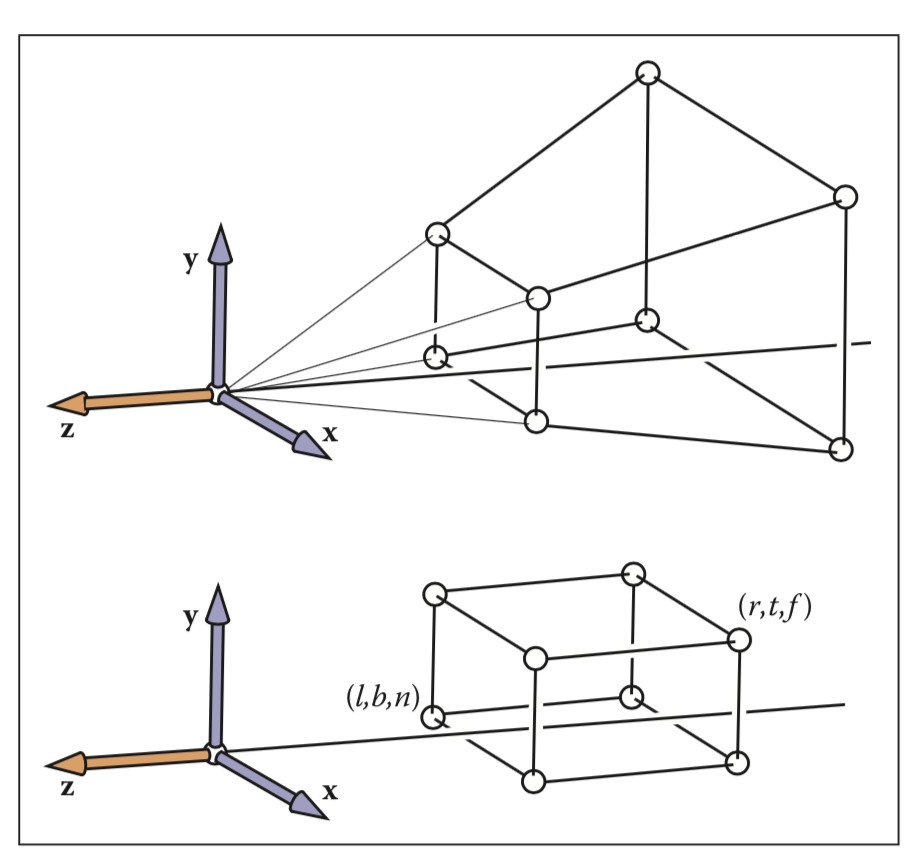
\includegraphics[width=2in]{perspective_projection_1}
        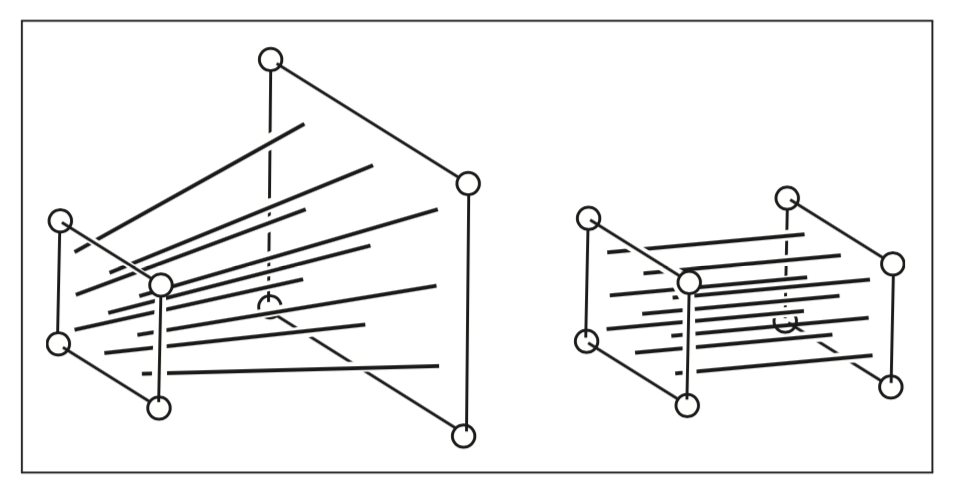
\includegraphics[width=3in]{perspective_projection_2}
        \caption{perspective projection maps line thorugh origin/eye to a line parallel to z-axis}
        \end{center}
    \end{figure}
    To convert screen coordinate plus $z$ back to the original space, we can apply the inverse of projective projection
    \[
        \bP^{-1} = 
        \begin{pmatrix}
            \frac{1}{n} & 0 & 0 & 0 \\
            0 & \frac{1}{n} & 0 & 0 \\
            0 & 0 & 0 & 1 \\
            0 & 0 & -\frac{1}{fn} & \frac{n+f}{fn} \\
        \end{pmatrix}
        \sim
        \begin{pmatrix}
            f & 0 & 0 & 0 \\
            0 & f & 0 & 0 \\
            0 & 0 & 0 & fn \\
            0 & 0 & -1 & n+f \\
        \end{pmatrix}
    \]
    The \underline{perspective projection matrix} maps perspective view volume to canonical view volume
    \[
        \bM_{per} = \bM_{orth} \bP = 
        \begin{pmatrix}
            \frac{2n}{r-l} & 0 & \frac{l+r}{l-r} & 0 \\
            0 & \frac{2n}{t-b} & \frac{b+t}{b-t} & 0 \\
            0 & 0 & \frac{f+n}{n-f} & \frac{2fn}{f-n} \\
            0 & 0 & 1 & 0 \\
        \end{pmatrix}
    \]
    To sum up,
    \[
        \begin{pmatrix}
            x_{pixel} / w_{pixel} \\
            y_{pixel} / w_{pixel} \\
            z_{ordered} / w_{pixel}\\ 
            1 \\
        \end{pmatrix}
        \sim
        \begin{pmatrix}
            x_{pixel} \\ y_{pixel} \\ z_{ordered} \\ w_{pixel}
        \end{pmatrix}
        = 
        (\bM_{vp} \bM_{orth} \bP \bM_{cam})
        \begin{pmatrix}
            x \\ y \\ z \\ 1
        \end{pmatrix}    
    \]
    note we need to divide by the homogeneous coordinate $w$ if perspective projection $\bM_{per}$ is included. 
    \item \bheading{properties of perspective transform} perspective transform preserves straight lines, planes, and triangles, and preserves the ordering of the points.
    \item \bheading{field of view} although we can specify any window $(l,r,b,t)$ and distance to plane $n$, we can have a simpler system where we 
    \begin{enumerate}
        \item look through the center of the window ($l=-r$ and $b=-t$)
        \item pixels are square and we want no distortion in the image ($nx / ny = r / t)$
    \end{enumerate}
    So pixel count $n_x, n_y$, (verticle) field-of-view $\theta$, and distance to plane $n$ defines the viewing window.
    \[
        \tan \frac{\theta}{2} = \frac{t}{|n|}    
    \]
    \Fig{fov}{0.5}{1}{field-of-view $\theta$ is the angle from bottom of the screen to the top of the screen}
\end{enumerate}


\section{\linkbook{167}{The Graphics Pipeline}}

\begin{enumerate}
    \item \bheading{the graphics pipeline} object-order rendering cosiders each object and find pixels that it could have an effect on. The proces of finding all pixels in an image occupied by an object is called \underline{rasterization}. object-order rendering can also be called rendering by rasterization. This sequence of operations in called the graphics pipeline. It is more effient.
    \begin{enumerate}
        \item interactive rendering via hardware for speed (OpenGL, Direct3D)
        \item film production rendering for quality (RenderMan)
    \end{enumerate}
    Steps are 
    \begin{enumerate}
        \item \heading{vertex processing} incoming vertices transformed by modeling, viewing, projection transformation which maps them from original coordinate into screen space. Color, surface normal, texture are also transformed as needed.
        \item \heading{rasterization} converts continuous representation of object to discrete pixels
        \item \heading{fragment processing} compute a color and depth for each fragment. shading operations
        \item \heading{fragment blending} compute final cover by combining fragments that overlapped each pixel, i.e. pick colo of fragment with smallest depth 
    \end{enumerate}
    \item \bheading{rasterization} In essence, rasterization converts continuous representation of objects to a discrete representation with pixels. The rasterizer enumerates pixels covered by the primitives and it interpolates values, called attributes, across the primitive. The output of the rasterizer is a set of fragments, one for each pixel covered by the primitive. Each fragment (lives) at a particular pixel and carries its own set of attribute values
    \item \bheading{line drawing} given implicit function 
    \[
        f(x,y) = 
        (y_0 - y_1)x + (x_1 - x_0)y + x_0y_1  - x_1y_0 = 0    
    \]
    assuming $x_0 < x_1$ and the slope $m = (y_1-y_0)/(x_1-x_0) \in (0,1]$. The midpoint algorithm keep drawing pixels from left to right and move upward in the $y$-direction if $f(x+1,y+0.5)<0$, i.e. the line passes over the midpoint of $(x+1,y)$ and $(x+1,y+1)$
    \item \bheading{triangle rasterization} In 2D, given $\bp_0, \bp_1, \bp_2$ in screen coordinates, we can draw triangle and fillin color with barycentric coordinates
    \[
        \bc = \alpha \bc_0 + \beta \bc_1 + \gamma \bc_2    
    \]
    where $\bc_0,\bc_1,\bc_2$ are color of triangle vertices. This is called Gouraud interpolation
    \item \bheading{A simple 2D pipeline} rasterization followed by blending stage where each fragment simply overwrites value of the previous one. This is the typical API for interfaces, graphing libraries
    \item \bheading{A minimal 3D pipeline} To draw 2D objects in 3D, simply follow the 2D pipeline with one addition: in vertex processing stage the incoming vertex positions are multiplied by the modeling, camera, projection, and viewport mtraices, resulting in screen-space triangles drawn in the same way as if they'd been specified directly in 3D. Use \textbf{painter's algorithm} to get the correct occlusion relationship, i.e. primitives are draw in back-to-front order. However, the drawbacks are 
    \begin{enumerate}
        \item cannot handle triangles that intersect one another
        \item several triangles can be arranged in an occlusion cycle
        \item sorting primitives by depth is slow
    \end{enumerate}
    \Fig{painters_drawbacks}{0.4}{1}{Drawback's of painter's algorithm}
    \item \bheading{use z-buffer for hidden surfaces} for each pixel, allocate a \textbf{depth buffer}, or z-buffer to store the closest distance of fragments that have been drawn so far. In the fragment blending stage, fragments with distance larger than the depth buffer is thrown away. This requires each fragment to carry a depth, which is computed by interpolation of $z$-coordinates. Thereare precision issues with $z$-buffer.$z$ buffer are nonnegative integers instead of float for memory speed reasons. 
    \item \bheading{per-vertex shading} idea is we want 3D objects to be drawn with shading, using the same illumination euqation used for image-order rendering. These equation requries a light direction, eye direction and surface normal to compute the color of a surface. Idea is 
    \begin{enumerate}
        \item application provides normal vectors at each vertex
        \item positions and color of lights are provided separately
        \item at each vertex, the direction to the viewer and direction to each lights are computed based on positions of the camera, lights, and vertex.
    \end{enumerate}
    the shading equation is evaluated to compute a color, which is passed onto the rasterizer as the \textbf{vertex color}. Per-vertex shading is called \textbf{Gouraud shading}. Usually, computation of vertex color is in a coordinate system orthonormal when viewed in the world space, e.g. the eye space. per-vertex shading has the disadvantage of not producing details in shading that are smaller than the primitives used to draw the surfaces, since it computes shading once for each vertex and never in between vertices.
    \item \bheading{per-fragment shading} To avoid interpolation artifacts associated with per-vertex shading, we can avoid interpolating colors by performing shading computations after the interpolation in the fragment stage. Geometric information needed for shading is passed through the rasterizer as attributes, so the vertex stage must coordinate with fragment stage to prepare the data appropriately. One approach is to interpolate eye-space surface normal and eye-space vertex positions.
    \item \bheading{texture mapping} textures are images that are used to add extra detail to the shading of surfaces that would otherwise look too homogeneous and artificial. Idea is each time shading is computed, read one values used in the shading computation, e.g. diffuse color, from the texture instead of attribute values attached to the geometry. This is called \textbf{texture lookup} the shading code specifies a \textbf{texture coordinate}
    \item \bheading{shading frequency} 
    \begin{enumerate}
        \item \heading{low shading frequency} shading with large-scale features can be evalauted fairly infrequently and interpolated
        \item \heading{high shading frequency} shading that produces small-scale features, such as sharp highlights or detailed textures. Most likely the shading frequency needs to be at least one shading sample per pixel
    \end{enumerate}
\end{enumerate}


\section{\linkbook{250}{Signal Processing}}
\section{\linkbook{250}{Surface Shading}}


\section{\linkbook{250}{Texture Mapping}}
\section{\linkbook{440}{17 Using Graphics Hardware}}


\begin{enumerate}
    \item \bheading{graphics hardware} hardware necessary to quickly render 3D objects using specialized rasterization-based hardware architectures. CPU can be programmed with OpenCL and CUDA
    \item \bheading{heterogeneous multiprocessing} 
\end{enumerate}

 


\end{document}
